\documentclass[twoside]{article}

\usepackage{aistats2020}

\usepackage{multirow}
\usepackage{enumitem}
\usepackage{graphicx}
\usepackage[utf8]{inputenc} % allow utf-8 input
\usepackage[T1]{fontenc}    % use 8-bit T1 fonts
\usepackage{hyperref}       % hyperlinks
\usepackage{url}            % simple URL typesetting
\usepackage{booktabs}       % professional-quality tables
\usepackage{amsmath,amssymb} 
\usepackage{amsthm}    % blackboard math symbols
\usepackage{nicefrac}       % compact symbols for 1/2, etc.
\usepackage{microtype}      % microtypography
\usepackage{bm}
\usepackage{subfig}
\usepackage[english]{babel}
\usepackage{algorithm}
%\usepackage{algorithmic}
\usepackage{appendix}

\theoremstyle{plain}
\newtheorem{thm}{Theorem}[section]
\newtheorem{lem}{Lemma}
\newtheorem{prop}{Proposition}
\newtheorem{pro}{Property}
\newtheorem{assumption}{Assumption}

\theoremstyle{definition}
\newtheorem{defn}{Definition}
\newtheorem{cor}{Corollary}
\newtheorem{example}{Example}
\newtheorem{rmk}{Remark}

\input macros.tex
\usepackage{dsfont}

\usepackage{multirow}
\usepackage{algpseudocode,algorithm}
\algnewcommand\algorithmicinput{\textbf{Input:}}
\algnewcommand\algorithmicoutput{\textbf{Output:}}
\algnewcommand\INPUT{\item[\algorithmicinput]}
\algnewcommand\OUTPUT{\item[\algorithmicoutput]}

\DeclareMathOperator*{\minimize}{minimize}



\usepackage{mathtools}
\mathtoolsset{showonlyrefs}
\newcommand*{\KeepStyleUnderBrace}[1]{%f
  \mathop{%
    \mathchoice
    {\underbrace{\displaystyle#1}}%
    {\underbrace{\textstyle#1}}%
    {\underbrace{\scriptstyle#1}}%
    {\underbrace{\scriptscriptstyle#1}}%
  }\limits
}
\usepackage{xr}
\externaldocument{tensor_regression_supp}

% If your paper is accepted, change the options for the package
% aistats2020 as follows:
%
% \usepackage[accepted]{aistats2020}
%
% This option will print headings for the title of your paper and
% headings for the authors names, plus a copyright note at the end of
% the first column of the first page.

% If you set papersize explicitly, activate the following three lines:
%\special{papersize = 8.5in, 11in}
%\setlength{\pdfpageheight}{11in}
%\setlength{\pdfpagewidth}{8.5in}

% If you use natbib package, activate the following three lines:
%\usepackage[round]{natbib}
%\renewcommand{\bibname}{References}
%\renewcommand{\bibsection}{\subsubsection*{\bibname}}

% If you use BibTeX in apalike style, activate the following line:
%\bibliographystyle{apalike}

\begin{document}

% If your paper is accepted and the title of your paper is very long,
% the style will print as headings an error message. Use the following
% command to supply a shorter title of your paper so that it can be
% used as headings.
%
%\runningtitle{I use this title instead because the last one was very long}

% If your paper is accepted and the number of authors is large, the
% style will print as headings an error message. Use the following
% command to supply a shorter version of the authors names so that
% they can be used as headings (for example, use only the surnames)
%
%\runningauthor{Surname 1, Surname 2, Surname 3, ...., Surname n}

\twocolumn[

\aistatstitle{Generalized tensor response regression with multi-sided covariates}

\aistatsauthor{ Anonymous Author 1 \And Anonymous Author 2 \And Anonymous Author 3}

\aistatsaddress{ Unknown Institution 1 \And  Unknown Institution 2 \And Unknown Institution 3 } ]

\begin{abstract}
We consider the problem of tensor-valued regression given covariates on a set of modes. Such data problems arise frequently arise in applications such as neuroimaging, network analysis, and spatial-temporal modeling. We propose a new family of tensor response regression models that incorporate covariate information, and obtain the theoretical accuracy guarantees. An efficient alternating updating algorithm is further developed. Our proposal handles a broad range of data types, including continuous, count, and binary observations. Through simulation and application to two real datasets, we demonstrate the outperformance of our approach over the state-of-art. \end{abstract}

\section{Introduction}

Many contemporary scientific and engineering studies collect multi-way array data, a.k.a.\ tensor, accompanied by additional covariates. For example, in neuro-imaging analysis, researchers measure brain connections from a sample of individuals with the goal to identify the brain edges affected by age and gender. In social network analysis, how to explain the connection (e.g. community, transitive, etc.) by attributable of both nodes. %ee demonstration plot. 
In this article, we provide a general treatment to these seemingly different problems.


\begin{figure*}
\begin{center}
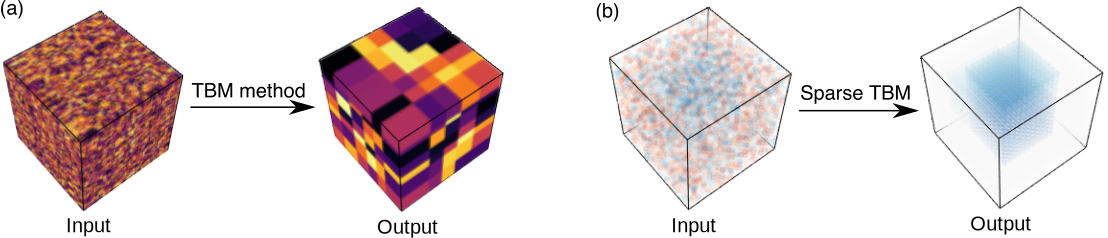
\includegraphics[width=17cm]{demo.pdf}
  \end{center}
\caption{Examples of tensor regression with multi-sided covariates. (a) Spatio-temproal growth model. (b) Network population model.}
  \end{figure*}


%{\bf Comparison with other models}\\
%Our model is related to, but fundamentally different from, several lines of existing work.\\
%{\bf Unsupervised tensor}. supervised learning. \\
%{\bf Tensor-predictor regression} multilinear in coefficients. \\
%{\bf Tensor-response regression} multilinear in coefficient vs. multilinear in covariates. \\
%{\bf Generalized linear model}. In the high-dimensions both $p$ and $n$ increase while $p \leq d$. This is the case we consider. Classical GLM fixes $p$. Compared to Gaussian model, the log-likelihood is not strictly convex in the linear predictor. We allow various types of dependent variable. 



\section{Preliminaries}

We begin by reviewing basic properties on tensors~\cite{kolda2009tensor}. We use $\tY=\entry{y_{i_1,\ldots,i_K}}\in \mathbb{R}^{d_1\times \cdots\times d_K}$ to denote an order-$K$ $(d_1,\ldots,d_K)$-dimensional tensor. The multilinear multiplication of a tensor $\tY\in\mathbb{R}^{d_1\times \cdots\times d_K}$ by matrices $\mX_k=\entry{x_{i_k,j_k}^{(k)}}\in\mathbb{R}^{s_k\times d_k}$ is defined as
\[
\tY \times_1\mX_1\ldots \times_K \mX_K=\entry{\sum_{i_1,\ldots,i_K}y_{i_1,\ldots,i_K}x_{i_1,j_1}^{(1)}\ldots x_{i_K,j_K}^{(K)}},
\]
which results in an order-$K$ tensor $(s_1,\ldots,s_K)$-dimensional tensor. For ease of notation, we use shorthand notion $\tY\times\{\mX_1,\ldots,\mX_K\}$ to denote the above product. A higher-order tensor can be reshaped into a lower-order representation. We let $\text{vec}(\cdot)$ to denote the operation that reshapes a tensor into a vector, and $\text{Unfold}_k(\cdot)$ the operation that reshapes a tensor along mode-$k$ into a matrix of size $d_k$-by-$\prod_{i\neq k}d_i$. The Tucker rank of an order-$K$ tensor $\tY$ is defined as a length-$K$ vector $\mr=(r_1,\ldots,r_K)$, where $r_k$ is the rank of matrix $\text{Unfold}_k(\tY)$. 


For any two tensors $\tY=\entry{y_{i_1,\ldots,i_K}}$, $\tY'=\entry{y'_{i_1,\ldots,i_K}}$ of identical order and dimensions, their inner product is defined as $\langle \tY, \tY'\rangle =\sum_{i_1,\ldots,i_K}y_{i_1,\ldots,i_K}y'_{i_1,\ldots,i_K}$. The Frobenius norm of tensor $\tY$ is defined as $\FnormSize{}{\tY}=\langle \tY,\ \tY \rangle^{1/2}$; it is the Euclidean norm of $\tY$ regarded as an $\prod_k d_k$-dimensional vector. We use lower-case letters, e.g.,\ $a,b,c$, for scalars and vectors, upper-case boldface letters, e.g., $\mA,\mB,\mC,$ for matrices, and calligraphy letter, e.g.\ $\tA, \tB, \tC,$ for tensors of order 3 or greater. We denote by $\mI_n$ the identity the $d \times d$ identity matrix. 


\section{Motivation and model}\label{sec:model}
Let $\tY=\entry{y_{i_1,\ldots,i_K}}\in\mathbb{R}^{d_1\times \cdots\times d_K}$ denote an order-$K$ data tensor of interest. Suppose we observe covariates on some of the $K$ modes. Let $\mX_k\in\mathbb{R}^{d_k\times p_k}$ denote the available covariates on the mode-$k$, where $p_k\leq d_k$. We propose the following multilinear structure for the mean tensor. Specifically, 
\begin{align}\label{eq:tensormodel}
&\mathbb{E}(\tY|\mX_1,\ldots,\mX_K)=f(\Theta),\ \text{with}\\
&\Theta =\tB\times\{\mX_1,\ldots,\mX_K\} ,
\end{align}
where $f(\cdot)$ is a known link function, $\Theta\in\mathbb{R}^{d_1\times \cdots\times d_K}$ is the linear predictor, $\tB\in\mathbb{R}^{p_1\times \cdots p_K}$ is the parameter tensor of interest, and $\times$ denotes the tensor Tucker product. The choice of link function depends on the distribution of the response data. Some common choices are identity link for Gaussian tensor, logistic link for binary tensor, and log link for Poisson tensor. We give three concrete examples of tensor regression model that arises in practice. 

\begin{example}[Spatio-temporal growth model]
Let $\tY=\entry{y_{ijk}}\in\mathbb{R}^{d \times m\times n}$ denote the pH measurements of $d$ lakes at $m$ levels of depth and for $n$ time points. Suppose the sampled lakes belong to $q$ types, with $p$ lakes in each type. Let $\{\ell_j\}_{j\in[m]}$ denote the sampled depth levels and $\{t_k\}_{k\in[n]}$ the time points. Assume the expected pH trend in depth is a polynomial of order $r$ and that the expected trend in time is a polynomial of order $s$. Then, the spatio-temporal growth model can be represented as
\begin{equation}\label{eq:time}
\mathbb{E}(\tY|\mX_1,\mX_2,\mX_3)=\tB\times\{\mX_1,\mX_2,\mX_3\},
\end{equation}
where $\tB\in\mathbb{R}^{p\times (r+1)\times (s+1)}$ is the coefficient tensor of interest, $\mX_1=\text{blockdiag}\{\mathbf{1}_p,\ldots,\mathbf{1}_p\}\in \{0,1\}^{d\times p}$ is the design matrix for lake types, 
\[
\mX_2=
\begin{pmatrix}
1 & \ell_1&\cdots &\ell^{r}_1\\
1 & \ell_2&\cdots &\ell^{r}_2\\
\vdots &\vdots&\ddots&\vdots\\
1&\ell_{m}&\cdots&\ell^{r}_{m}
\end{pmatrix},\
\mX_3=
\begin{pmatrix}
1 & t_1&\cdots &t^{s}_1\\
1 & t_2&\cdots &t^{s}_2\\
\vdots &\vdots&\ddots&\vdots\\
1&t_{n}&\cdots&t^{s}_{n}
\end{pmatrix}
\]
are the design matrices for spatial and temporal effects, respectively. Clearly, the spatial-temporal model is a special case of our tensor regression model, with covariates on each of the three modes. The model~\eqref{eq:time} can be viewed as a higher-order extension of the classical ``growth curve'' models for matrix data in the context of factorial design~\cite{gabriel1998generalised,potthoff1964generalized,srivastava2008estimation}. 

\end{example}
\begin{example}[Network population model] 
Network response model is recently developed in the context of neuroimanig analysis. The goal is to study the relationship between network-valued response and the individual covariates. Suppose we observe $n$ i.i.d.\ observations $\{(\mY_i, \mx_i): i=1,\ldots,n\}$, where $\mY_i\in\{0,1\}^{d\times n}$ is the brain connectivity network on the $i$-th individual, and $\mx_i\in\mathbb{R}^p$ is the individual covariate such as age, gender, cognition, etc. The network-response model~\cite{rabusseau2016low, zhang2018network} has the form
\begin{equation}\label{eq:network}
\text{logit}(\mathbb{E}(\mY_i|\mx_i))=\tB\times_3\mx_i, \quad \text{for }i=1,\ldots,n
\end{equation}
where $\tB\in \mathbb{R}^{d\times d\times p}$ is the coefficient tensor of interest. 

The model~\eqref{eq:network} is a special case of our tensor-response model, with covariate on one of the three modes. Specifically, let $\tY\in\{0,1\}^{d\times d\times n}$ denote the response tensor by stacking $\{\mY_i\}$ together along the 3$^\text{rd}$ mode and $\mX=[\mx_1,\ldots,\mx_n]\in\mathbb{R}^{p\times n}$, then model~\eqref{eq:network} can be expressed as 
\[
\text{logit}(\mathbb{E}(\tY|\mX))=\tB\times_3 \mX=\tB\times\{\mI_d, \mI_d, \mX\}.
\]
 \end{example}
 
 \begin{example}[Dyadic data with node attributes] Dyadic data consist of measurements on pairs of objects or under a pair of conditions. Common examples include networks and graphs. Let $\tG=(V,E)$ denote a network, where $V=[n]$ is the node set of the graph, and $E\subset V\times V$ is the edge set. We also observe covariate $x_i\in\mathbb{R}^p$ associated to each $i\in V$. The network $\tG=(V,E)$ is described by the following matrix model. The edge connects the two vertices $i$ and $j$ independently of the others, and the probability of connection is modeled as
\begin{equation}\label{eq:edge}
 \text{logit}(\mathbb{P}((i,j)\in E)=\mx^T_i\mB\mx_j=\langle \mB, \mx^T_i\mx_j\rangle.
 \end{equation}
The above model has demonstrated its success in explaining higher-order dependence, such as transitivity, balance, and clusterability in the network data~\cite{hoff2005bilinear}. We show that our tensor regression model incorporates the dyadic model as a special case. Let $\tY=\entry{y_{ij}}$ where $y_{ij}=\mathds{1}_{(i,j)\in E}$. Define $\mX=[\mx_1,\ldots,\mx_n]\in\mathbb{R}^{p\times n}$. Then, the dyadic model~\eqref{eq:edge} can be expressed as
 \[
 \text{logit}(\mathbb{E}(\mY|\mX))=\tB\times\{\mX,\mX\}.
 \]
\end{example}

In the above three examples and many other studies, researchers are interested in uncovering the variation in the data tensor that are explained by the covariates. The regression coefficient $\tB$ in our model model~\eqref{eq:tensormodel} serves this goal by revealing the effects that are attributable to covariates and the interaction thereof.  %Estimation accuracy can be improved by restricting $\tB$ to a parameter space of lower dimension. 
%Without any structure on the coefficient tensor $\tB$: \emph{A naive approach is to regress the tensor entry, one at a time, on the covariates, and this model is repeatedly fitted for each tensor element.} Though this approach is scalable, it suffers from two drawbacks: (1) ignore the interdependence among entries in the tensor and (2) suffers from the multiplicity issue. %To allow the structure among ..
Furthermore, we assume that the coefficient tensor $\tB$ admits a low-rank Tucker decomposition,
\begin{equation}\label{eq:rank}
\tP=\{\tB\in\mathbb{R}^{p_1\times \cdots \times p_K}: r_k(\tB)\leq r_k \text{ for } k\in[K]\},
\end{equation}
where $r_k(\tB)\leq p_k$ is the Tucker rank of the tensor at mode $k$. The low-rank assumption is plausible in many scientific applications. In brain imaging analysis, for instance, it is often believed that the nodes can be classified into fewer communities, and the numbers of communities are much smaller than the dimension. Moreover, the low-rank structure encourages the shared information across tensor entries, thereby greatly improving the estimation stability.  


Our tensor regression model is able to incorporate covariates on some or all modes, whenever available. Without loss of generality, we denote by $\tX=\{\mX_1,\ldots,\mX_K\}$ the covariates in all modes and treat $\mX_k=\mI_{d_k}$ if the mode-$k$ has no (informative) covariate. Then, the final form of our tensor regression model can be written as:
\begin{align}\label{eq:tensormodel}
&\mathbb{E}(\tY|\tX)=f(\Theta),\quad \Theta =\tB\times\{\mX_1,\ldots,\mX_K\},\notag\\
&\text{where}\ \text{rank}(\tB)=(r_1,\ldots,r_K),
\end{align}
where $\tB\in\mathbb{R}^{p_1\times \cdots\times p_K}$ is the low-rank coefficient tensor of interest, and the entries of $\tY$ are independent conditional on $\tX$. We comment that other forms of tensor low-rankness is also possible, and here we choose Tucker rank for parsimony. Similar models can be derived using other notions of low-rankness based on CP decomposition~\cite{hitchcock1927expression} and train decomposition~\cite{oseledets2011tensor}. 
%Note that the key assumption in the model is the low-rankness of the tensor form. The low-rank structure in~\eqref{eq:rank} implies that the coefficient tensor can be expressed as $\tB=\tC\times\{\mM_1,\ldots, \mM_K\}$. Then, our tensor regression model~\eqref{eq:tensormodel} is equivalent to
%\[
%f(\mathbb{E}(\tY|\mX_1,\ldots,\mX_K))=\tC\times\{\mX_1\mM_1,\ldots,\mX_k\mM_k\}.
%\]
%The goal is to find a joint dimension reduction of $\tY$ and $\mX_K$ such that the unexplained variation in the mean tensor. The factorization is restricted to the space spanned by $\mX_k$. Here $\mX_1\mM_1$ can be interpreted as the latent covariates that explains the variation in the response tensor. The core tensor $\tC$ collects the interaction effects of latent covariates across the $K$ modes.  

\section{Rank-constrained likelihood-based estimation}
We develop a likelihood-based procedure to estimate the tensor. The exponential family is a flexible framework for different data types. In a classical GLM with a scalar response $y$ and covariate $\mx$, the density is expressed as:
\[
p(y|\mx, \boldsymbol{\beta})=c(y)\exp\left({y\theta- b(\theta) \over \phi}\right)\ \text{with}\ \theta=\boldsymbol{\beta}^T\mx,
\]
where $b(\cdot)$ is a known function, $\theta$ is the linear predictor, $\phi>0$ is the dispersion parameter, and $c(\cdot)$ is a known normalizing function. The choice of link functions depends on the data types and on the observation domain of $y$, denoted $\mathbb{Y}$. For example, the observation domain for continuous data is $\mathbb{Y}=\mathbb{R}$, for count data $\mathbb{Y}=\mathbb{N}$, and for binary data, $\mathbb{Y}=\{0,1\}$. 
Note that the canonical link function $f$ is chosen to be $f(\cdot)=b'(\cdot)$. Table~1 summarizes the canonical link functions for common types of distributions. 

\begin{table}
\begin{tabular}{c|ccc}
Data type &Gaussian & Poisson& Bernoulli\\
\hline
Domain $\mathbb{Y}$& $\mathbb{R}$&$\mathbb{N}$&$\{0,1\}\\
 $b(\theta)$&$\theta^2/2$& $\exp(\theta)$&$\log (1+\exp(\theta))$\\
 link $f(\theta)$&$\theta$&$\exp(\theta)$&$(1+\exp(-\theta))^{-1}$
\end{tabular}
\caption{Canonical link functions for various distribution types.}
\end{table}

In our context, the entries in the response tensor $y_{ijk}$ conditional on $\theta_{ijk}$ are independent drawn from exponential family. The quasi log-likelihood of~\eqref{eq:tensormodel} is equal (ignoring constant) to Bregman distance between $\tY$ and $b'(\Theta)$:
\begin{align}
\tL_{\tY}(\tB)&=\langle \tY, \Theta \rangle - \sum_{i_1,\ldots,i_K} b(\theta_{i_1,\ldots,i_K}),\\
\text{where}\ \Theta&=\tB\times\{\mX_1,\ldots,\mX_K\}.
\end{align}
We assume that we have an additional information on an upper bound $\alpha>0$ such that $\mnormSize{}{\Theta}\leq \alpha$. This is the case for many applications we have in mind such as brain imaging where fiber connections are bounded. We propose a constrained maximum likelihood estimator for the coefficient tensor:
\begin{equation}\label{eq:MLE}
\hat \tB=\argmax_{\text{rank}(\tB)= \mr, \mnormSize{}{\Theta(\tB)}\leq \alpha} \tL_{\tY}(\tB).
\end{equation}
In the following theoretical analysis, we assume the rank $\mr=(r_1,\ldots,r_K)$ is known and fixed. The adaptation of unknown $\mr$ will be addressed in Section~\ref{sec:tuning}. 


\subsection{Statistical properties}
We assess the estimation accuracy using the deviation in the Frobenius norm. For the true coefficient tensor $\trueB$ and its estimator $\hat \tB$, define
\[
\text{Loss}(\trueB,\ \hat \tB)=\FnormSize{}{\trueB- \hat \tB}^2.
\]

\begin{figure*}
\begin{center}
\includegraphics[width=17.5cm]{algorithm.pdf}
  \end{center}
  \end{figure*}
  
 In modern applications, the response tensor and covariates are often large-scale. We are particularly interested in the high-dimensional region in which both $d_k$ and $p_k$ diverge; i.e.\ $d_k\to \infty$ and $p_k\to\infty$, while ${p_k\over d_k} \to \gamma_k \in[0,1)$. As the size of problem grows, and so does the number of unknown parameters. As such, the classical maximum likelihood estimation  theory does not directly apply. We leverage the recent development in random tensor theory and high-dimensional statistics to establish the error bounds of the tensor estimation. 

\begin{assumption}\label{ass}We make the following assumptions:
\vspace{-.5cm}
\begin{enumerate}
\item [A1.] There exist two positive constants $c_1, c_2>0$ such that $c_1\leq \sigma_{\min}(\mX_k)\leq  \sigma_{\max}(\mX_k)\leq c_2$ for all $k\in[K]$. Here $\sigma_{\text{min}}(\cdot)$ and $\sigma_{\text{max}}(\cdot)$ denotes the smallest and largest singular values, respectively.
\item [A2.] There exist two positive constants $L,\ U>0$ such that $L\leq \text{Var}(y_{i_1,\ldots,i_K}|\tX, \tB)\leq U$ uniformly over the parameter space $\tP$. 
\end{enumerate}
\end{assumption}
Both assumptions are fairly mild. Assumption A1 guarantees the non-singularity of the covariates, and Assumption A2 ensures the log-likelihood $\tY(\Theta)$ is strictly concave in the linear predictor $\Theta$. Note that, for exponential family, $\text{Var}(y_{i_1,\ldots,i_K}|\tX,\tB)=b''(\theta_{i_1,\ldots,i_K})$~\cite{mccullagh1989generalized}, so the Assumption A2 can also be replaced by $L\leq b''(\theta) \leq U$ for all $|\theta|\leq \alpha$, where $\alpha$ is the upper bound of the linear predictor $\theta$. 

  
\begin{thm}[Statistical convergence]\label{thm:main}
Consider a generalized tensor regression model with multi-sided covariates $\tX=\{\mX_1,\ldots,\mX_K\}$. Suppose the entries in $\tY$ are independent realizations of an exponential family distribution, and $\mathbb{E}(\tY|\tX)$ follows the low-rank tensor regression model~\eqref{eq:tensormodel}. Under Assumption~\ref{ass}, there exist two absolute constants $C_1, C_2>0$, such that, with probability at least $1-\exp(-C_1\sum_k p_k)$, 
\begin{equation}\label{eq:bound}
\text{Loss}(\trueB,\ \hat \tB) \leq C_3\sum_k p_k,
\end{equation}
where $C_3=C_3(\mr)={1\over C^{2K}_2U}{\prod_k r_k \over \max_k r_k}>0$ is a constant that does not depend on the dimensions $\{d_k\}$ and $\{p_k\}$. 
\end{thm}

To gain further insight on the bound~\eqref{eq:bound}, we consider a special case when dimensions are equal at each of the modes, i.e., $d_k=d$, $p_k=\gamma d$, $\gamma\in [0,1)$ for all $k\in[K]$, and the covariates $\mX_k$ are Gaussian design matrices with i.i.d.\ $N(0,\sigma^2)$ entries. To put the result in the context of Theorem~\ref{thm:main}, we define rescaled covariates $\check \mX_k={1\over \sqrt{d}}\mX_k$, and note that the singular values of $\check \mX_k$ are bounded in $1\pm \sqrt{\gamma}$. The bound~\eqref{eq:bound} then reduces to $\tO({p\over d^K})$ for the estimated coefficient under the original, unscaled covariates $\{\mX_k\}$. Therefore, our estimation is consistent as the dimension grows, and the convergence becomes especially favorably as we have more modes in the tensor data. 

As immediate applications, we obtain the convergence rate for the three examples mentioned in Section~\ref{sec:model}. Without loss of generality, we assume that the singular values of the (informative) covariates $\mX_k$ are scaled as $\sqrt{d_k}$. 
\begin{cor}[Spatio-temporal growth model] The estimated type-by-time-by-level tensor converges at the rate $\tO\left({p+r+s\over dmn}\right)$ where $p\leq d$, $r\leq m$ and $s\leq n$. The estimation achieves consistency as long as the dimension grows in either of the three modes.
\end{cor}

\begin{cor} [Network population model] The estimated node-by-node-by-covariate tensor converges at the rate $\tO\left({2d+p\over d^2n}\right)$ where $p\leq n$. The estimation achieves consistency as the number of individuals or the number of nodes grows. 
\end{cor}

\begin{cor} [Link model with node attributes] The estimated covariate-by-covariate matrix converges at the rate $\tO\left({p\over d^2}\right)$ where $p\leq d$. Again, our estimation achieves consistency as the number of nodes grows. 
\end{cor}

We conclude this section by providing the prediction accuracy for the response tensor.  

\begin{thm} [Prediction error]
Assume the same set-up as in Theorem~\ref{thm:main}. Let $\mathbb{P}_{\tY_{\text{true}}}$ and $\mathbb{P}_{\hat \tY}$ denote the distribution of $\tY$ given the $\trueB$ and $\hat \tB$, respectively. Similarly, let $\mathbb{E}(\tY|\tX)$ and $\widehat{\mathbb{E}(\tY|\tX)}$ denote, respectively, the true and estimated mean. We have, with probability at least $1-\exp(C_1\sum_k p_k)$,
\begin{align}
&\text{KL}(\mathbb{P}_{\tY_{\text{true}}},\ \mathbb{P}_{\hat \tY})\leq C_4 \sum_k p_k,\ \text{and}\\
&\text{Loss}\left(\mathbb{E}(\tY|\tX),\ \widehat{\mathbb{E}(\tY|\tX)}\right)\leq C_5 \sum_k p_k,
\end{align}
where $C_4, C_5>0$ are two constants that do not depend on the dimension $\{d_k\}$ and $\{p_k\}$.
\end{thm}

\subsection{Comparison with existing work}\label{sec:compare}
In this section, we discuss the comparison between our method and previous work.  A fundamental feature of tensor-valued data is the statistical interdependence among entries, and one of our goals is to quantify this interdependence. 
%\newpage
%\subsubsection{Comparison between Gaussian and non-Gaussian models}
%Our earlier result gives the general bound with a constant factor $C$. The factor depends on the tensor order, rank, the distribution family, and the infinity norm bound. We now discuss its specific form for various distribution types of the response. We consider the special case when $d_1=\ldots=d_K=d$, $p_1=\ldots=p_K=p$, $r_1=\ldots=r_K=r$. The constant $C={2\over b''(\alpha)} \prod_k\sigma^{-1}_{\min}(\mX_k)$. For Bernoulli model with logistic link $b''(\alpha)={e^\alpha\over (1+e^\alpha)^2}$. The bound
%\[
%\text{Loss}(\trueB,\hat B)\leq {2\over c_1^2K}\min\left\{ {r^{K-1} e^\alpha\over (1+e^\alpha)^2} {p\over d^K},\ 2\alpha^2 \right\}.
%\]
%The $\alpha$ can be interpreted as the signal level. As $p\to\infty, d\to\infty, {p\over d} \to \gamma\in[0,1]$. For consistent estimation, we require $\tO(d^{-(K-1)})\ll \alpha\ll \tO((K-1)\log d)$. 

%\resizebox{.5\textwidth}{!}{
%\begin{tabular}{c|ccc}
%Type & $\alpha \lesssim  d^{-(K-1)/2}$ & $ d^{-(K-1)/2} \ll \alpha\ll \tO((K-1)\log d)$ & $\alpha\gg (K-1)\log d$\\
%\hline
%Bernoulli& $2\alpha^2$ & $$& $e^{\alpha - (K-1)\log d}$ \\
%\end{tabular}}

%\newpage
\section{Numerical implementation}
\subsection{Alternating optimization}
In this section, we introduce an efficient algorithm to solve~\eqref{eq:MLE}. The objective function $\tL_{\tY}(\tB)$ is concave in $\tB$ when the link $f$ is canonical link function. However, the feasible set $\tP$ is non-convex, and thus the optimization~\eqref{eq:MLE} is a non-convex problem. We utilize a Tucker factor representation of coefficient tensor $\tB$, and turn the optimization into a block-wise convex problem. 

Specifically, write the rank-$\mr$ decomposition of coefficient tensor $\tB$ as
\begin{equation}\label{eq:tucker}
\tB=\tC\times \{\mM_1,\ldots,\mM_K\},
\end{equation}
where $\tC\in\mathbb{R}^{r_1\times\cdots\times r_K}$ is a full-rank core tensor, $\mM_k\in\mathbb{R}^{p_k\times r_k}$ are factor matrices whose columns are orthogonal. Estimating $\tB$ amounts to finding both the core tensor $\tC$ and the factor matrices $\mM_k$'s. Then, the optimization~\eqref{eq:MLE} can be written as $(\hat \tC, \{\hat \mM_k\})=\arg\max \tL_{\tY}(\tC, \mM_1,\ldots,\mM_K)$, where
\begin{align}\label{eq:obj}
\tL_{\tY}(\tC, \mM_1,\ldots,\mM_K )&=\langle \tY, \Theta\rangle -\sum_{i_1,\ldots,i_K}b(\theta_{i_1,\ldots,i_K}),\\
\text{with } \Theta&=\tC\times\{\mM_1\mX_1,\ldots,\mM_K\mX_K\}.
\end{align}
The decision variables in the above objective function consist of $K+1$ blocks of variables, one for the core tensor $\tC$ and $K$ for the factor matrices $\mM_k$'s. We notice that, if any $K$ out of the $K+1$ blocks of variables are known, then the optimization with respect to the last block of variables reduced to a simple GLM. This observation suggests that we can iteratively update one block at a time while keeping others fixed. Specifically, suppose the core tensor and the factor matrix $\mM_k$ are known for $k=1,\ldots,K-1$. It turns out that last factor matrix $\mM_K$ can be solved in a row-by-row fashion via $d_k$ separate GLMs. To see this, let $\tC^{(t)}$ denote the core tensor at the $t$-th iteration,  $\mM^{(t)}_k$ the $k$th factor matrix for $k\in[K-1]$ at the $t$-th iteration, and define
\[
\mX^{(t)}_{-K}=\tC^{(t)}\times \{ \mM^{(t)}_1\mX_1,\ \ldots,\ \mM^{(t)}_{K-1}\mX_{K-1}\},
\]
Then, the objective~\eqref{eq:obj} implies that the $i$-th row of $\mM^{(t)}_K$ is the ``regression coefficient'' for a GLM whose response vector is $\text{vec}(\tY(:,\ :, \ i))\in\mathbb{R}^{d_{-K}}$ and covariate matrix is $\text{Unfold}_K(\mX_{-K}^{(t)})\in\mathbb{R}^{d_{-K} \times r_K}$, where $d_{-K}\stackrel{\text{def}}{=}\prod_{k\in[K-1]}d_k$. The property of separation by row allows us to leverage state-of-art GLM solvers and parallel processing to achieve computational efficiency. After each iteration, we rescale the core tensor $\tC^{(t+1)}$ subject to the infinity norm constraint. This post-processing in principle may not guarantee the monotonic increase of the objective, but we found that in our experiment this simple post-processing appears to be good enough for a desirable solution. The full algorithm is described in Algorithm~1.



\subsection{Rank selection, missing data handling}\label{sec:tuning}
Before concluding this section, we briefly comment on two implementation details. First, Algorithm~1 takes the rank $\mr$ as an input. Estimating an appropriate rank given the data is of practical importance. We propose to use Bayesian information criterion (BIC) and choose the rank that minimizes BIC; i.e.
\begin{align}\label{eq:BIC}
\hat \mr&=\argmin_{\mr=(r_1,\ldots,r_K)} \text{BIC}(\mr)\\
&=\argmin_{\mr=(r_1,\ldots,r_K)}\left[-2\tL_{\tY}(\hat \tB)+p_e(\mr)\log \left(\prod_k d_k\right) \right],
\end{align}
where $p_e(\mr)\stackrel{\text{def}}{=}\sum_k (p_k-r_k-1)r_k+\prod_k r_k$ is the effective number of parameters in the model. We choose $\hat \mr$ that minimizes $\text{BIC}(\mr)$ via grid search. Our choice of BIC aims to balance between the goodness-of-fit for the data and the degree of freedom in the population model. We test its empirical performance in Section~\ref{sec:simulation}.  

Second, when some response entries $y_{i_1,\ldots,i_K}$ are missing, we replace the objective function by $\tL_{\tY}$ $= \sum_{(i_1,\ldots,i_K)\in\Omega}\left(y_{i_1,\ldots,i_K}\theta_{i_1,\ldots,i_K}-b(\theta_{i_1,\ldots,i_K})\right)$, where $\Omega\subset[d_1]\times \cdots \times [d_K]$ is the index set of non-missing entries. That is, we model the observed response entries and exclude the missing entries in the fitting. Similar strategy has been used for classical (unsupervised) Tucker and CP tensor decomposition with missing data~\cite{acar2010scalable,wang2018learning,wang2017tensor}. In the presence of missing response, we modify line 7 in Algorithm 1 by fitting GLMs to the data for which $y_{i_1,\ldots,i_K}$ are observed. This approach requires there are no entirely missing slice, e.g.\ in the form of $\tY(:,\ :,\ k)$ for order-3 tensors. We regard this as a fairly mild condition akin to the coherence condition as in the completion literature~\cite{candes2009exact,ghadermarzy2018learning}.


\section{Simulation}\label{sec:simulation}
We evaluate the empirical performance of our generalized tensor regression through simulations. We consider order-3 tensors with a range of distribution types. The coefficient tensor $\tB$ is generated using the factorization form~\eqref{eq:tucker} where both the core and factor matrices are drawn i.i.d.\ from Uniform[0,1]. The linear predictor is then simulated as $\tU=\tB\times\{\mX_1,\mX_2,\mX_3\}$, where $\mX_k$ is either an identity matrix (i.e. no covariate available) or Gaussian random matrix with entries i.i.d.\ from $N(0,\sigma^2)$. Without loss of generality, we set $\sigma^2=d_k^{-1/2}$ to ensure the singular values of $\mX_k$ are bounded as $d_k$ increases. We rescale $\tU$ such that $\mnormSize{}{\tU}=1$. Conditional on the linear predictor $\tU=\entry{u_{ijk}}$, the entries in tensor $\tY=\entry{y_{ijk}}$ are drawn independently according to one of the following three probabilistic models:

\begin{enumerate}[itemsep=0pt,topsep=0pt]
\item[(a)] (Gaussian). Continuous data $y_{ijk}\sim N\left(\alpha u_{ijk}, 1\right)$.
\item[(b)] (Poisson). Count data $y_{ijk}\sim\text{Poi}\left( e^{\alpha u_{ijk}}\right)$.
\item[(c)] (Bernoulli). Binary data $y_{ijk}\sim \text{Ber}\left( {e^{\alpha u_{ijk}} \over 1+e^{\alpha u_{ijk}}}\right)$.
\end{enumerate}
Here $\alpha>0$ is a scalar controlling the magnitude of the linear predictor. In each simulation study, we report the mean squared error for the coefficient tensor averaged across $n_{\text{sim}}=30$ replications. 

The first experiment assesses the selection accuracy of our BIC criterion~\eqref{eq:BIC}. We consider the balanced situation where $d_k=d$, $p_k=0.4d_k$ for $k=1,2,3$. We set $\alpha=10$, $\alpha=4$, and consider various combinations of dimension $d$ and rank $\mr=(r_1,r_2,r_3)$. For each combination, we simulate tensor data following Gaussian, Bernoulli, and Poisson models. We then minimize BIC over $\mr$ using a grid search over three dimensions. We set the hyper-parameter $\alpha$ to infinity in the fitting, which essentially poses no prior on the coefficient magnitude. Table~\ref{tab:rank} reports the selected rank averaged over $n_{\text{sim}}=30$ replicates for Gaussian and Poisson models. (The results for Bernoulli model is shown in the Supplements.) We found that when $d=20$ the selected rank is slightly smaller than the true rank, and the accuracy increases immediately when the dimension increases to $d=40$. This agrees with our expectation, as in tensor regression, the sample size is related to the number of entries. A larger $d$ implies a larger sample size, so the BIC selection becomes more accurate. 


\begin{table}[t]
\resizebox{.48\textwidth}{!}{
\begin{tabular}{|c|cc|cc|}
\hline
%&\multicolumn{4}{c}{Dimension}\\
True Rank &\multicolumn{2}{c|}{Dimension (Gaussian tensors)}&\multicolumn{2}{c|}{Dimension (Poisson tensors)}\\
$\mr$& $d=20$  &$d=40$&$d=20$ &$d=40$\\
\hline
$(3,\ 3,\ 3)$&$(2.1,\ 2.0,\ 2.0)$&$({\bf 3},\ {\bf 3},\ {\bf 3})$&$(2.0,\ 2.2,\ 2.1)$&$({\bf 3},\ {\bf 3},\ {\bf 3})$\\
$(4,\ 4,\ 6)$&$(3.2,\ 3.1,\ 5.0)$&$({\bf 4},\ {\bf 4},\ {\bf 6})$&$({\bf 4.0},\ {\bf 4.0},\ 5.2)$&$({\bf 4},\ {\bf 4},\ {\bf 6})$\\
$(6,\ 8,\ 8)$&$(5.1,\ 7.0,\ 6.9)$&$({\bf 6},\ {\bf 8},\ {\bf 8})$&$(5.0,\ 6.1,\ 7.1)$&$({\bf 6},\ {\bf 8},\ {\bf 8})$\\
\hline
\end{tabular}
}
\caption{Performance for rank selection via BIC. Bold number indicates no significant difference between the estimate and the ground truth, based on a $z$-test with a level 0.05.}\label{tab:rank}
\end{table}

The second experiment evaluates the accuracy when covariates are available on all modes. We set $\alpha=10, d_k=d, r_k=r\in\{2,4,6\}$ and increase $d$ from 25 to 50. Our theoretical analysis suggests $\hat \tB$ has a convergence rate $\tO(d^{-2})$ in this setting. Figure~1 plots the estimation error versus the ``effective sample size'' $d^2$ under three different distribution models. We found that the empirical RMSE decreases roughly at the rate of $1/d^2$, which is consistent with our theoretical ascertainment. We also observed that coefficients with higher ranks tend to yield higher estimation errors, as reflected by the upward shift of the curves as $r$ increases. Indeed, a larger $r$ implies higher model complexity, thus increasing the difficulty of the estimation. Similar behaviors can be observed in the non-Gaussian data in Figure~2b-c. 

\begin{figure}[H]
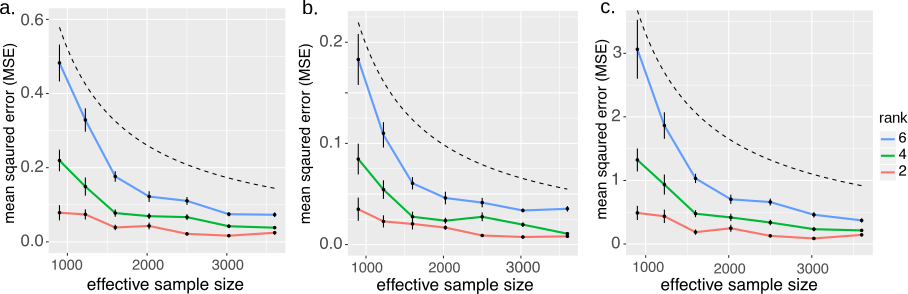
\includegraphics[width=8.5cm]{..//../code/binary_tucker/team/figure/dimension.pdf}
\caption{Estimation error against effective sample size. The three panels depicts the MSE when the response tensor is generated form (a) Gaussian (b) Poisson and (c) Bernoulli models. Each solid curve corresponds to a fixed rank. The dashed curve corresponds to $\tO({1/d^2})$.}
\end{figure}

The third experiment investigates our model's ability in handling correlation among coefficients. We mimic the scenario of brain imaging analysis. A sample of $d_3=50$ networks are simulated, one for each individual. Each network measures the connections between $d_1=d_2=20$ brain nodes. We simulate $p=5$ covariates for the $50$ individuals. These covariates may represent, for example, age, gender, cognitive score, etc. Recent study~\cite{robinson2015dynamic} has suggested that brain connectivity networks often exhibit community structure represented as a collection of subnetworks, and each subnetwork is comprised of a set of spatially distributed brain nodes. To accommodate this structure, we utilize the popular stochastic block model to generate the effect size. Specifically, we created $r$ blocks among the nodes by randomly assigning each node to a cluster with uniform probability. Edges within a same block are assumed to share the same covariate effects, where the effects are drawn i.i.d.\ from $N(0,1)$. We then applied our tensor regression model to the network data using the BIC-selected rank. Note that in this case, the true model rank is unknown; the rank of a $r$-block matrix is bounded by but not necessarily equal to $r$~\cite{zeng2019multiway}. 

Figure~\ref{fig:glm} compares the MSE of our model with a classical GLM approach. A classical GLM is to regress the dyadic edges, one at a time, on the covariates, and this model is repeatedly fitted for each edge. This approach, however, does not account for the correlation structure among the edges. As we can see in Figure~\ref{fig:glm}, out tensor regression method achieves significant error reduction in all three models considered. The outer-performance is more apparent in the presence of large communities, and even in the less structured case ($\sim 20/15=1.33$ nodes per block), our method still outer-performs GLM. This is because the low-rankness in our modeling automatically identifies the shared information across entries. By a data-driven rank selection, our method is able to achieve accurate estimation with improved interpretability. 


\begin{figure}[t]
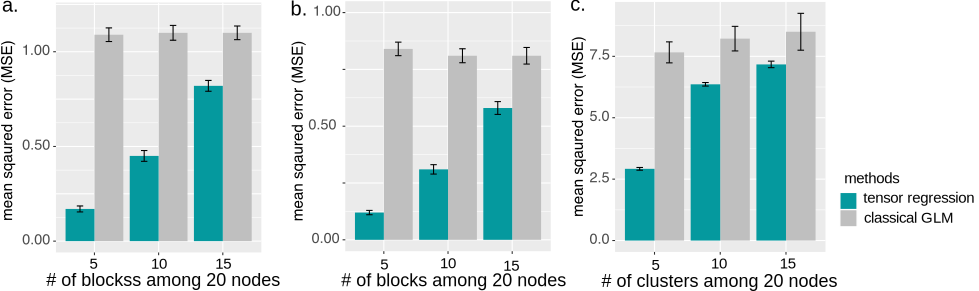
\includegraphics[width=8.5cm]{..//../code/binary_tucker/team/figure/comparison.pdf}
\caption{Performance comparison when the population network admit block structure. The three panels depicts the MSE when the response tensor is generated form (a) Gaussian (b) Poisson and (c) Bernoulli models. The $x$-axis represents the number of blocks in the networks. }\label{fig:glm}
\end{figure}


\section{Data analysis}
We apply our tensor regression model to two real datasets. The first application concerns the modeling of brain network population in response to individual attributes (i.e.\ covariate on one mode), and the second application focuses on multi-relational network analysis with dyadic attributes (i.e.\ covariates on two modes). 

\subsection{Human Connectome Project (HCP)}
The Human connectome project (HCP) aims to build a ``network map'' that characterizes the anatomical and functional connectivity within healthy human brains. 
We took a subset of HCP data that consists of 136 brain structural networks, one for each individual. Each brain network is represented as a 68-by-68 binary matrix, where the entries encode the presence or absence of fiber connections between the 68 brain regions. Individual covariates are also available. For simplicity of presentation, we consider four covariates: gender (65 females vs.\ 71 males), age 22-25 ($n=35$), age 26-30 ($n=58$), and age 31+ ($n=43$). The goal is to identify the connection edges that are affected by the individual covariates. A key challenge in brain network is that the edges are correlated; for example, two edges may stem out from a same brain region, and it is of importance to take into account the within-dyad dependence. 

We fitted the tensor regression model to the HCP data. The response is a binary tensor $\tY\in\{0,1\}^{68\times 68\times 136}$ and the covariates are of dimension 4 along the 3rd mode. The BIC selection suggests a rank $\mr=(10,10,4)$ with log-likelihood $\tL_{\tY}=-174654.7$. Figure~\ref{fig:brain} shows the top edges with high effect size, overlaid on the Desikan atlas brain template~\cite{desikan2006automated,xia2013brainnet}. For better interpretation, we utilized the sum-to-zero contrasts in the effects coding and depicted only the top 3\% edges with non-constant connections in the study sample. It is observed that the global connection exhibit clear spatial separation, and that the nodes within each 
hemisphere are more densely connected with each other (Figure~\ref{fig:brain}a). In particular, the superiortemproal (\emph{SupT}), middletemporal (\emph{MT}) and Insula are the top three popular nodes in the network. Interestingly, female brains displays higher inter-hemispheric connectivity, especially in the frontal, parental and temporal lobes (Figure~\ref{fig:brain}b). This is in agreement with a recent study showing that female brains are optimized for inter-hemispheric communication~\cite{ingalhalikar2014sex}. We also found several edges with declined connection in the group Age 31+. Notably, those edges involves Frontalpole (\emph{Fploe}), superiorfrontal (\emph{SupF}) and Cuneus nodes. The Frontalpole region has long been known for its importance in memory and cognition, and the declined fiber connections in Frontalpole node may suggests its anatomical change with age. 
\begin{figure}[t]
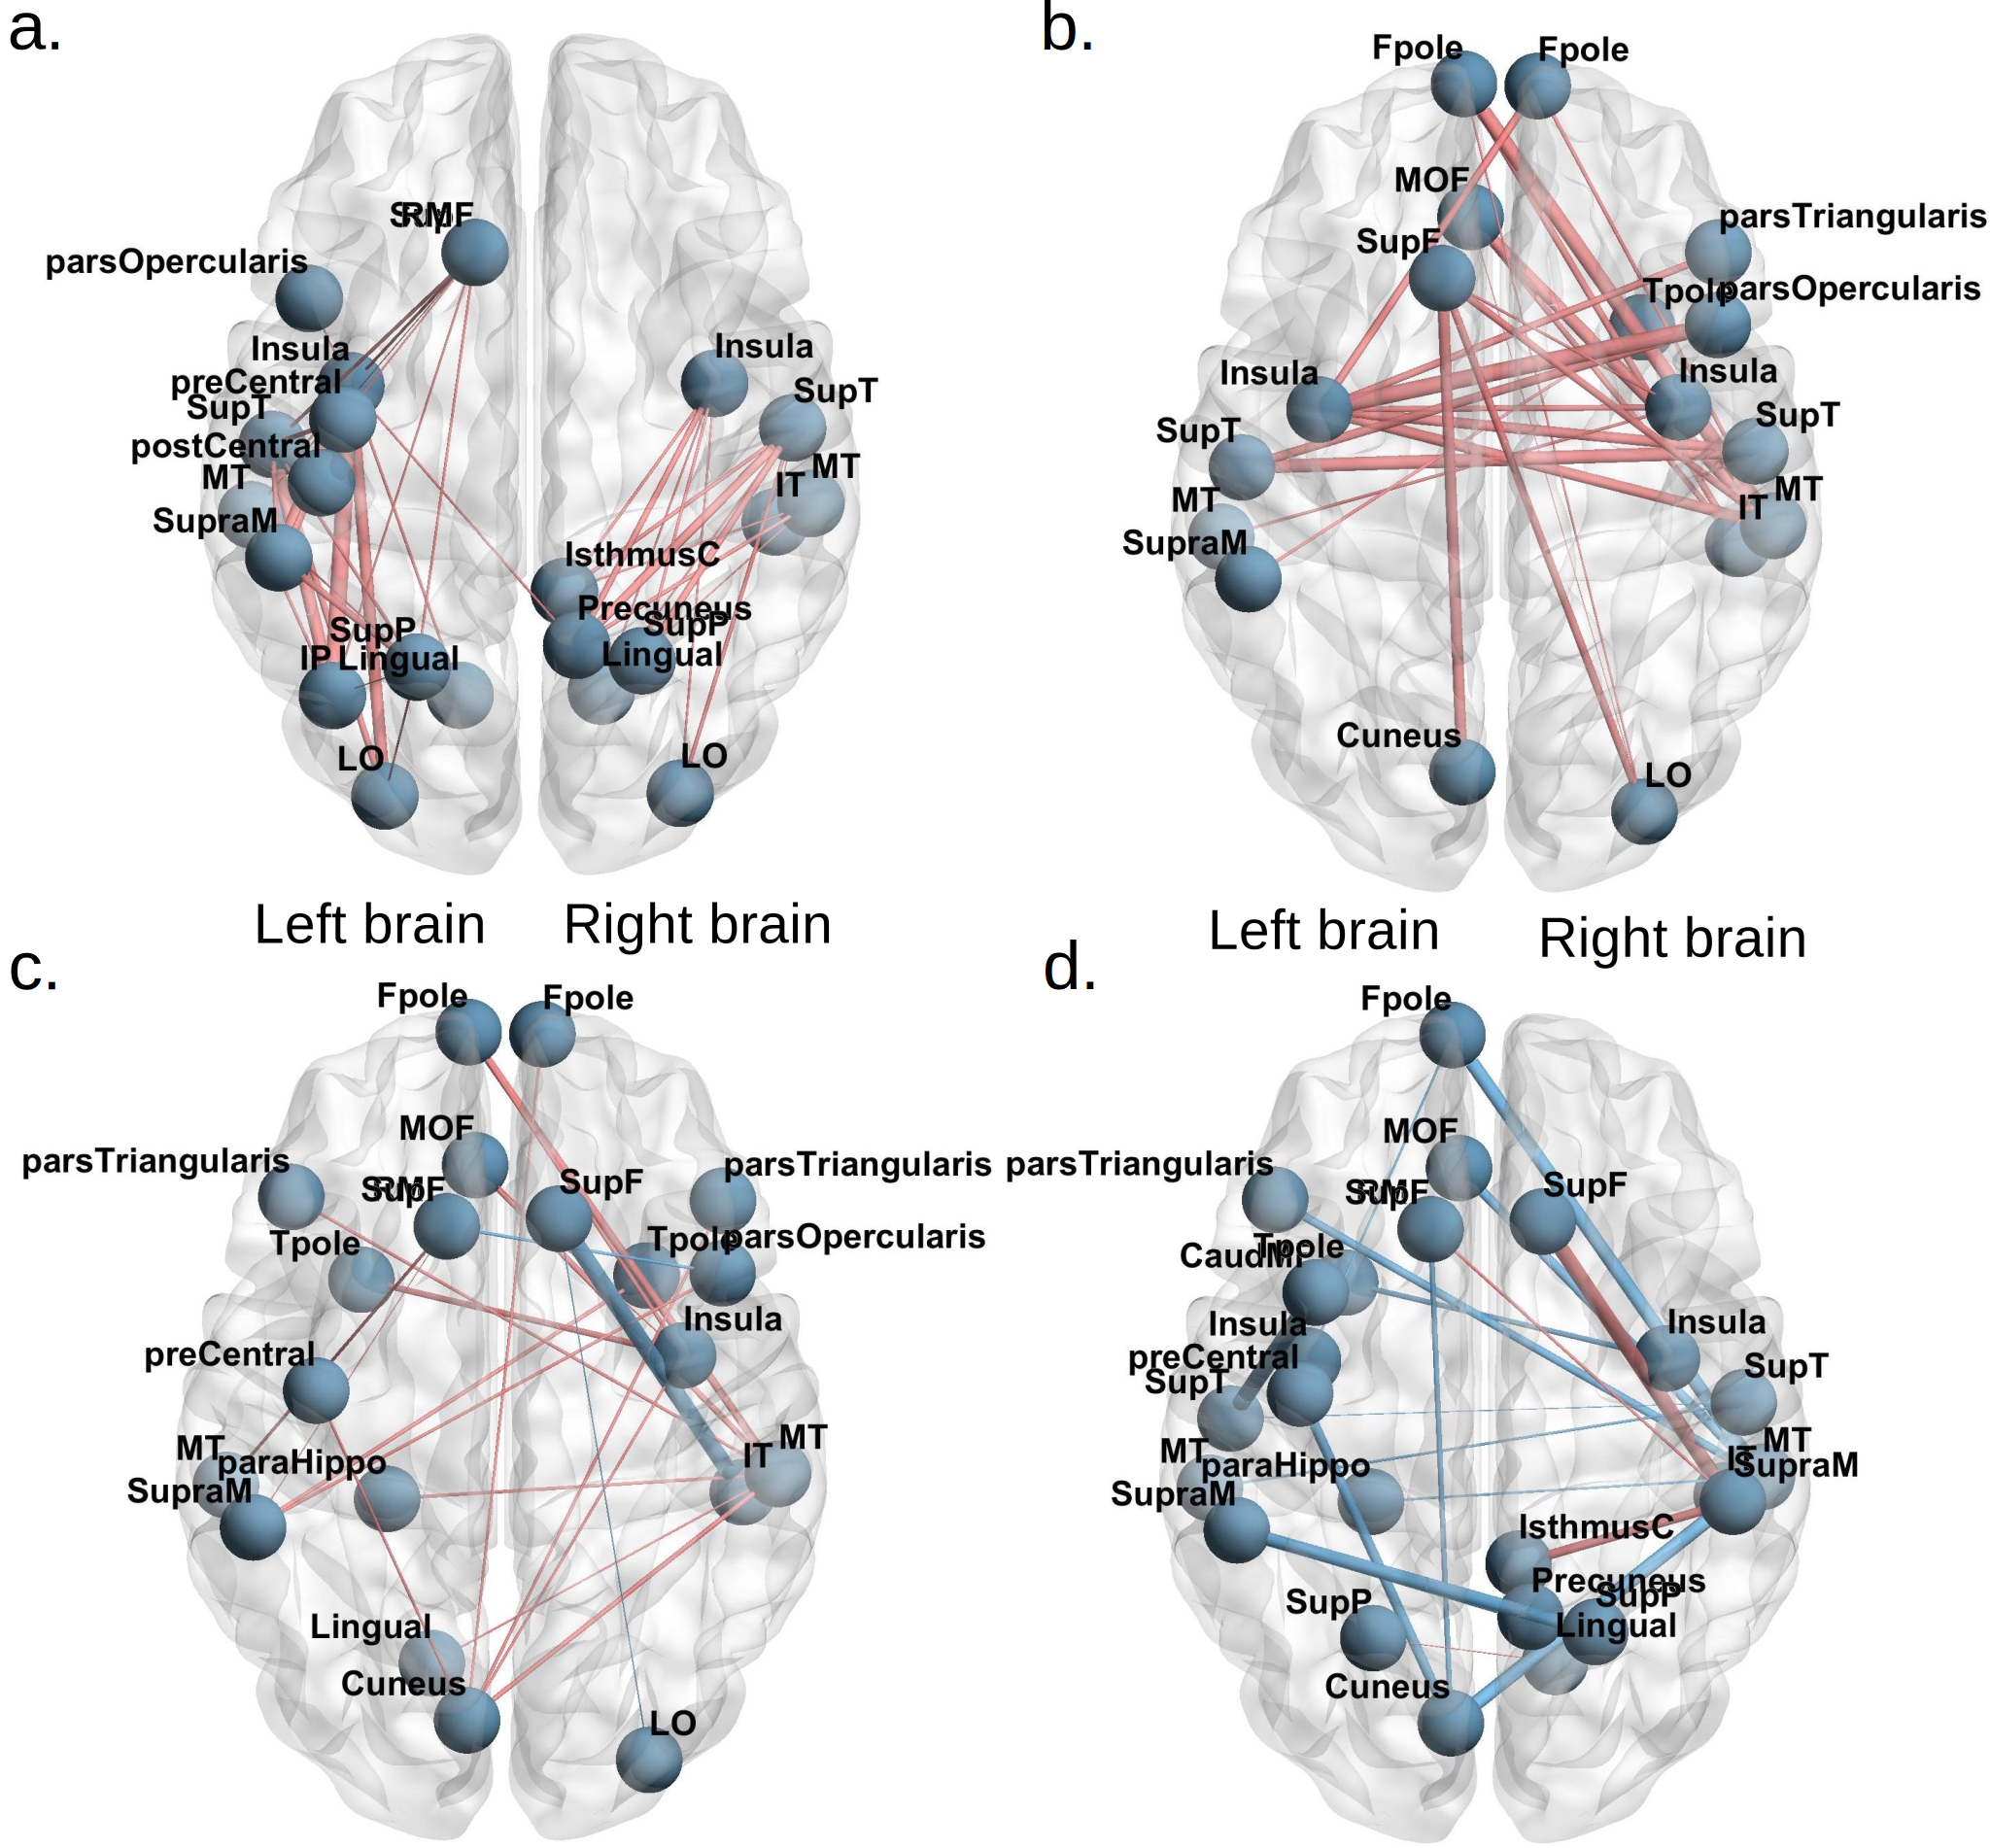
\includegraphics[width=8cm]{HCP.pdf}
\caption{Top edges with high effect size. (a) Global effect; (b) Gender effect; (c) Age 22-25; (c) Age 31+}\label{fig:brain}
\end{figure}

\subsection{Nations data}
The second application concerns the multi-relational network analysis with node-level attributes. We consider \emph{Nations} dataset~\cite{nickel2011three} which records 56 relations among 14 countries between 1950 and 1965. The multi-relational networks can be organized into a $14 \times 14 \times 56$ binary tensor, with each entry indicating the presence or absence of a connection, such as ``sending tourist to'', ``export'', ``import'', between countries. The 56 relations span the fields of politics, economics, military, religion, and so on. In addition, country-level attributes are also available, and we focus on the following six covariates: \emph{constitutional, catholics, lawngos, politicalleadership, geographyx}, and \emph{medicinengo}. The goal is to identify the variation in connections due to country-level attributes and interactions thereof. One of the key features is that the 56 relations are correlated, and we would like to take that into account in assessing the covariate effects. 

We applied our tensor regression model with two-sided covariates to the \emph{Nations} data. The multi-relational network $\tY\in\{0,1\}^{14\times 14\times 56}$ was treated as the response tensor, and the country attributes $\mM\in\mathbb{R}^{14\times 6}$ were treated as covariates in both the 1st and 2nd modes. The BIC criterion suggests a rank $\mr=(4,4,4)$ for the coefficient tensor $\tB\in\mathbb{R}^{6\times 6 \times 56}$. Supplementary Table S1 shows the $K$-mean clustering of the 56 relations based on the 3rd mode factor $\mM_3\in\mathbb{R}^{56\times 4}$. We found that the relations reflecting the similar aspects of international affairs are grouped together. In particular, Cluster I consists of political relations such as \emph{officialvisits, intergovorgs}, and \emph{militaryactions}; Clusters II and III are dominated by economical relations including \emph{economicaid, booktranslations, tourism, etc}; and Cluster IV represents the Cold War alliance blocs. The similarity among entities in each cluster suggests the plausibility of our dimension reduction. 

\begin{figure}[t]
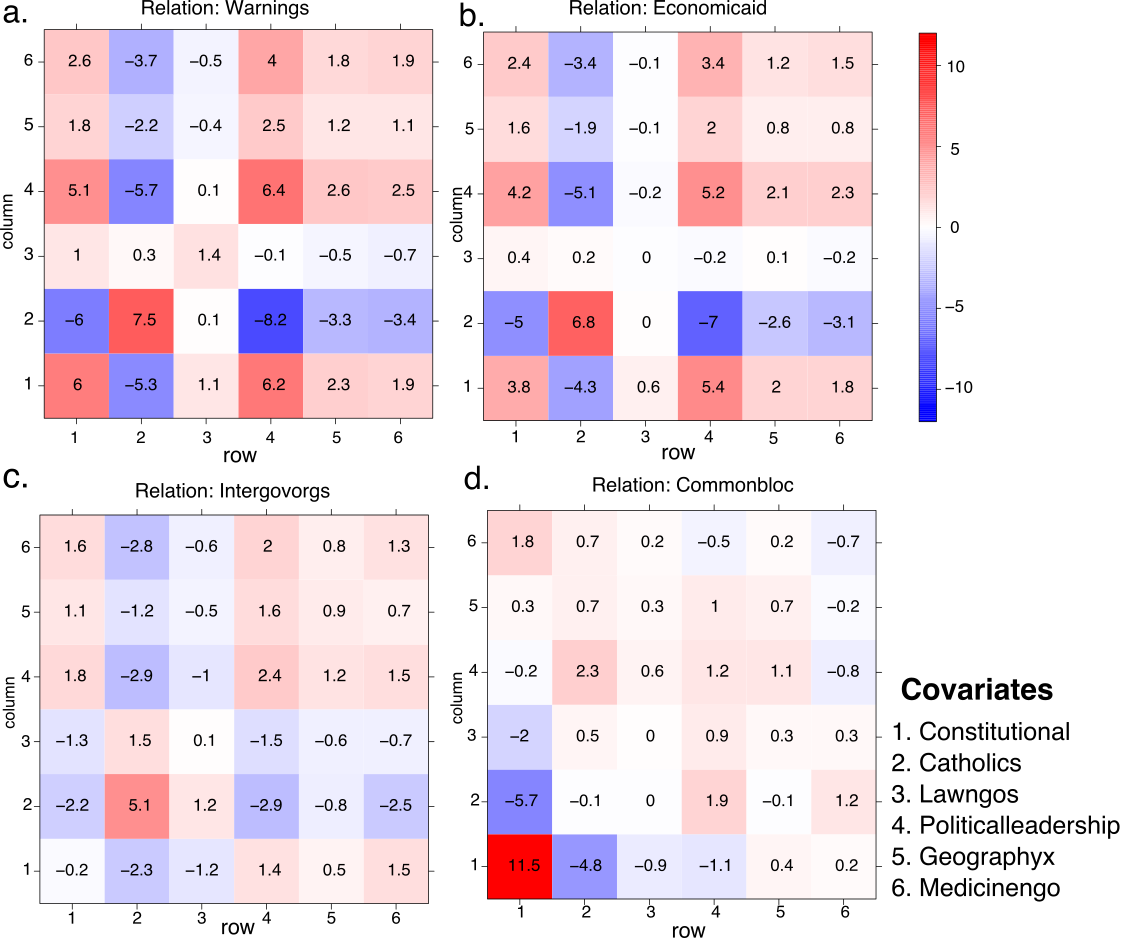
\includegraphics[width=7.5cm]{coef.pdf}
\caption{Estimated coefficient of country attributes towards the connection probability of relation type $k$.}\label{fig:est}
\end{figure}


To investigate how the dyadic attributes affect the connection, we depicted the estimated coefficients $\hat \tB=\entry{\hat b_{ijk}}$ for a few relation types (Figure~\ref{fig:est}). Note that entries $\hat b_{ijk}$ can be interpreted as the contribution, at the logit scale, of covariate pair $(i,j)$ ($i$th covariate for the ``sender'' country and $j$th covariate for the ``receiver'' country) towards the connection of relation $k$.  Several interesting findings emerge from the estimation. We found that relations belonging to a same cluster tend to have similar covariate effects. For example, the relations \emph{warnings} and \emph{ecnomicaid} were classified into Cluster II, and both exhibit similar covariate pattern (Figure~\ref{fig:est}a-b). Moreover, the diagonal entries $\hat \tB(i,i,k)$ tend to positively contribute to the connection. This is probably explained by the fact that countries with coherent attributes tend to interact more often than others. We also found that the \emph{constitutional} attributes are greatly associated with the \emph{commonbloc} relation, whereas such association is weaker for other relations (Figure~\ref{fig:est}d). This is not surprising, as the common block partition during Cold War is determined by capitalism vs.\ communism, which confounds with the \emph{constitutional} attributes. 

\section{Conclusions}
\bibliographystyle{unsrt}
\bibliography{tensor_wang}

\end{document}
